\section{Overview of Blockchain Naming Systems}
\label{sec:naming_systems}

\begin{table}
	\begin{tabular}{r l l}
		\toprule
		Name system & TLDs & Proxies \\
		\midrule
		Namecoin & .bit & BDNS (defunct), \\
		& & PeerName \\
		Emercoin & .lib, &  friGate, \\
		& .bazar, &  PeerName,\\
		& .coin, & OpenNIC \\
		& .emc & \\
		Handshake & \emph{any string} & hns.to, \\
		& & NextDNS, \\
		& & HDNS.io,\\
		& & BobWallet extension, \\
		& & LinkFrame extension \\
		ENS & .eth & eth.link, \\
		& & eth.limo \\
		Unstoppable & .crypto, & Brave browser, \\
		& .blockchain, & Opera browser, \\
		& .bitcoin, & Unstoppable browser, \\
		& .coin, & Unstoppable extension, \\
		& .nft, & Infura\\
		& .wallet, & \\
		& .888, & \\
		& .dao, & \\
		& .x, & \\
		& .zil & \\
		\bottomrule
	\end{tabular}
	\caption{Non-exhaustive selection of proxies, browsers, 
		and extensions 
		that can be used to access blockchain-based naming 
		systems.}
		%\randall{maybe should have a citation for each of these}}
	\label{tab:proxies_and_tlds}
\end{table}

In this section we present an overview of five blockchain-based naming 
systems, to provide background on how such systems work in detail. We select 
these systems based on their apparent popularity, as well as 
prior reports and literature that indicate some of them have already been 
abused by malware. These naming systems fall into two categories: systems built 
on naming-specific blockchains like Namecoin and Emercoin, whose purpose is 
primarily to store names and records, and systems built on general-purpose 
blockchains such as Ethereum, that are designed for purposes beyond naming 
systems. These systems also fall into two ``generations:'' Namecoin and 
Emercoin have existed since 2011 and 2013 
respectively~\cite{namecoin, emercoin}, while the Ethereum 
Name Service (ENS), Handshake, and Unstoppable 
Domains are more recent inventions (2017, 2018, and 2019, 
respectively~\cite{ens_website, handshake_website, 
first_ud_txn}). 

All of the blockchain-based naming systems we study differentiate their names 
from DNS domains by creating alternate top level domains, 
which we refer to as \emph{alt-TLDs} for brevity. A 
summary of the alt-TLDs used by each naming system is presented in 
Table~\ref{tab:proxies_and_tlds}. Handshake names are slightly different, since 
the goal of the Handshake project is to replace the DNS root zone and make any 
alt-TLD available for purchase --- see Section~\ref{sec:handshake} for more 
details.

%Although each of these systems are blockchain-based naming 
%systems, they differ in several key ways, which are relevant to how defenders 
%must treat them when they are abused by malware authors. We now summarize each 
%system in more detail.

\subsection{Naming-Specific Blockchains}

We study three naming systems that are built on 
naming-specific and eponymous blockchains: 
Namecoin, Emercoin, and Handshake. All of these blockchains 
are primarily designed to support their naming systems,  
rather than to create new cryptocurrencies or support arbitrary 
blockchain-native programs (``smart contracts''). Because 
these 
blockchains have such specific purposes, they differ 
from blockchains like Ethereum in two ways: they have fewer 
participants and users, and their transaction fees are much 
less expensive. Both properties have implications for 
defenders --- see Section~\ref{sec:accessing_records} 
for more details. 

\subsubsection{Namecoin and Emercoin}

Namecoin and Emercoin, which are both modified copies of Bitcoin, are 
the oldest blockchain-based naming systems. Both were 
intended as additions to traditional DNS: users registered domains that 
resolved to IP addresses, using records very similar to DNS 
records. Unfortunately, Namecoin and Emercoin have been subject to a large 
amount of abuse. Four years after Namecoin's launch, Kalodner et al. found that 
only 28 of the 120,000 domains registered in Namecoin had meaningful web 
content, and most domain registrations appeared to be 
squatting~\cite{kalodner_namecoin_2015}. 
In 2021, Casino et al. collected all of the IP addresses stored by Emercoin 
and Namecoin records, and submitted them to threat intelligence services 
including VirusTotal, Hybrid Analysis, Abuse.ch, and Pydnsbl (an aggregator of 
blocklists). They found that over 50\% of the IPs in Namecoin and Emercoin 
records had been flagged as malicious by at least one threat intelligence 
service~\cite{casino_unearthing_2021}. Furthermore, Casino et al. used a 
``poisoning'' approach to find IP addresses associated with malicious IPs, 
either because the two addresses were stored in the same 
wallet, a name resolved to both addresses at different times, 
or the same email was recorded in their records. This ``poisoning'' approach 
revealed that the vast majority of IP addresses in Namecoin and Emercoin 
records are connected in some way to malicious 
IPs~\cite{casino_unearthing_2021}. 
%While blocklists may 
%contain false positives, analysis of malware binaries has 
%also revealed dozens of hard-coded Emercoin and Namecoin 
%domains that are used to contact C2 servers, as well as DGAs 
%that generate Namecoin domains for the same 
%purpose~\cite{citations_needed}. 
Our own findings support the conclusion that these naming 
systems are still rife with abuse (Section~\ref{sec:b-root}). 

%The names registered in Namecoin and Emercoin have been well studied in 
%prior work, so we did not conduct our own study of them, 
%unlike the other three naming systems we study.


\subsubsection{Handshake}
\label{sec:handshake}
\begin{table}
	\begin{tabular}{lr}
		\toprule
		Record & Names with Record \\
		\midrule
		Default NS and GLUE4 records & 102,386 \\
		\hspace*{0.2in} No A records & 102,285\\
		\hspace*{0.2in} A 44.235.163.135 & 94 \\
		\hspace*{0.2in} A 52.43.158.89 & 4 \\
		\hspace*{0.2in} A 144.91.114.245 & 2 \\
		\hspace*{0.2in} A 1.1.1.1 & 1 \\
		Invalid name & 98,068 \\
		No record (null) & 845 \\
		TXT record & 138 \\
		\hspace*{0.2in} ``hello fx-wallet'' & 110 \\
		\hspace*{0.2in} Other & 28 \\
		Non-default NS record & 32 \\
		Non-default GLUE4 record & 11 \\
		Distributed storage address & 7 \\
		\midrule
		Total unique names & 201,458 \\
		Total records & 201,487 \\
		\bottomrule
	\end{tabular}
	\caption{Record types in the Handshake namespace.}
	\label{tab:handshake_records}
\end{table}

Handshake is a blockchain-based naming system that aims to replace the root DNS 
zone. It offers its users the ability to purchase nearly any 
string to 
use as an alt-TLD. Rather than selling second-level domains 
itself, Handshake allows its users 
to act as registrars who can sell their own domains. 
Handshake records are designed to store the NS records of traditional 
authoritative nameservers, rather than to replace DNS A, AAAA, or similar 
records. Handshake 
also allows users to 
store TXT records, which can contain the addresses for decentralized web 
hosting systems like Skynet~\cite{skynet} or IPFS~\cite{ipfs}. Malware 
operators could 
potentially use 
Handshake as a naming system to find C2 content stored in 
these distributed storage systems. Additionally, Handshake 
advertises themselves as ``the only naming blockchain with a lightweight 
recursive DNS resolver, which you can easily embed into 
browsers, apps, and devices''~\cite{namebase_access_handshake}. 
This lightweight resolver may be attractive to malware 
operators because it is 
small enough to be part of a malware payload.

%\randall{Summarize the .music debate and cite it somewhere.}

To get a sense for how people use Handshake, we collected a 
sample of approximately 201,000 recently registered Handshake 
names by scraping a Handshake block 
explorer.\footnote{https://e.hnsfans.com/names} 
We attempted to scrape these names 
directly from the Handshake blockchain, but were 
unsuccessful because the RPC 
provided by the Handshake client to collect registered names 
from a Handshake node is no 
longer functional~\cite{hns_rpc_too_big}. 
Table~\ref{tab:handshake_records} 
summarizes our findings. At the moment, Handshake names appear to be 
overwhelmingly utilized as speculative assets. Only 0.14\% of 
names in our sample had NS records that differed from the 
default. Of the names that kept the default nameserver and 
glue records, only 101 (0.05\%) eventually resolved to A records, 94 of 
which were for the same IP address (a nameserver run by Namebase). Nearly half 
of registered Handshake domains in our sample cannot be 
resolved by the HNS client, since they contain illegal characters like emojis 
or are solely composed of numbers: these names are nevertheless allowed to be 
created on the Handshake blockchain. We concluded that the Handshake system has 
not yet seen significant adoption by either licit users or malicious 
actors.

\subsection{Naming Systems on General Purpose Blockchains}

Two naming systems based on the Ethereum blockchain have 
arrived since 2017: the Ethereum Name 
Service (ENS) and Unstoppable Domains. These naming systems 
are possible because of Ethereum's innovation in the 
blockchain space: \emph{smart contracts.} Smart contracts 
are code that is embedded into the Ethereum 
blockchain. Any machine that runs an Ethereum ``full node'' 
can execute any 
smart contract. Each contract is identified by a 20-byte 
address, and makes its functions available through its 
Application Binary Interface (ABI). 
Thus, asking a smart contract to execute one of its functions 
is similar to 
making an RPC call, except that instead of one machine executing the code, 
every machine that receives the transaction must do so. 

Smart contracts can be used to implement key-value stores, which means they are 
well suited to act as naming 
systems. For example, in a simplified system, a user might wish to set the name 
``foo.crypto'' to resolve to the IP address 1.2.3.4. The user would create an 
Ethereum transaction that asks the key-value store's smart 
contract 
to call its ``set record'' function, with ``foo.crypto'' and 
``1.2.3.4'' as function inputs. 
This transaction is then broadcast to the Ethereum network, 
and every Ethereum 
node that receives it updates its own copy of the key-value store to include 
the new record. Reading from the key-value store works similarly to writing to 
it: any Ethereum node can return a correct response. 
%Implication: taking down 
%the host of a name on Ethereum is not possible without taking down every 
%Ethereum node. In contrast to IPFS, where only one machine stores the content 
%you're looking for, so taking it down might be a lot easier.
Notably, any transaction that causes a write costs a ``gas 
fee'' of Ethereum cryptocurrency. Gas fees are 
dependent on network 
congestion as well as other factors: they incentivize 
Ethereum node operators to execute smart contract code, which 
uses computing resources. In contrast, reading a 
smart contract's data does not cost a gas fee and does not 
create a transaction.

Interestingly, ENS and Unstoppable Domains are structured 
like DNS, but they are not necessarily being used as DNS 
replacements. The language and structure of both systems' 
smart 
contracts implies that they were 
modeled after DNS: for example, both systems use certain 
smart contracts 
as registries, and ENS even uses others as resolvers and 
registrars. However, users are primarily using these systems 
to map human-readable names to \emph{cryptocurrency wallet 
addresses} 
instead of IP addresses. While users can still store IP 
addresses, traditional domains, TXT records, or distributed 
storage system (DS) addresses, 
very few choose to do so. This may imply that C2 records containing IP 
addresses or DNS domains will stand out and be easier for defenders to detect.

\subsubsection{ENS}

\begin{table}
	\begin{tabular}{lrr}
		\toprule
		Resolver Name & Txns Setting Resolver & Address \\
		\midrule 
		Public Resolver 2 & 33,304 & \texttt{0x4976fb...} \\
		Public Resolver 1 & 2,736 & \texttt{0xDaaF96...} \\
		OpenSea ENS resolver & 482 & \texttt{0x9C4e9C...} \\
		ENS Old Public Resolver 2 & 440	& \texttt{0x226159...} \\
		Umbra: Stealth Resolver & 409 & \texttt{0xB37671...} \\
		\textit{unnamed PublicResolver} & 126 & \texttt{0xD3ddcC...} \\
		\textit{unnamed PublicResolver} & 103 & \texttt{0x5FfC01...} \\
		ENS Old Public Resolver 1 & 29 & \texttt{0x1da022...} \\
		\bottomrule
	\end{tabular}
	\caption{The ENS resolvers from which we collected a 
	sample of names and records.}
	\label{tab:ens_resolvers}
\end{table}

\begin{figure}[t]
	\centering
	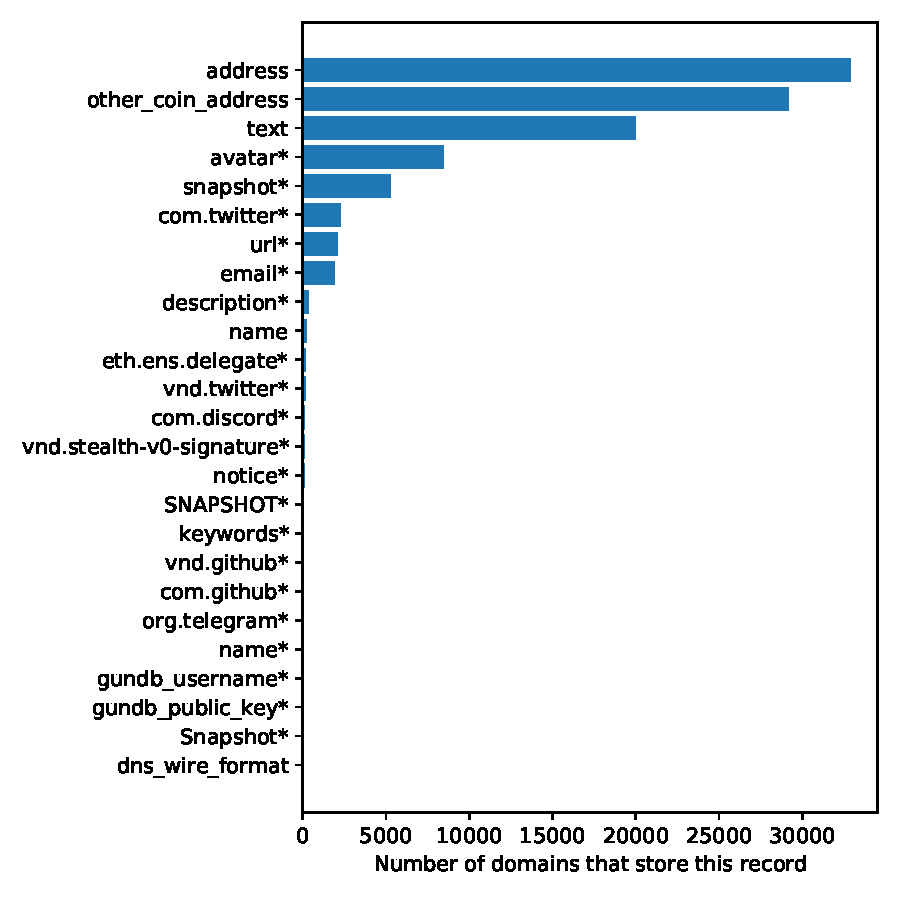
\includegraphics[width=3in]{figs/ens_names.pdf}
	\caption{Records stored by ENS names. *key within ``text'' record}
	\label{fig:ens_records}
\end{figure}

ENS names are registered (and resolved) in two steps involving two different 
smart contracts. First, a name must be registered using the ``ENS Registrar 
Controller'' smart contract, which accepts the human-readable name and the 
address of a contract to use as a ``resolver.'' Second, the 
resolver
contract must be updated with the name's records. To complicate matters, names 
are not handled in their human-readable forms after they are registered: 
instead, they are referred to by their keccak256 hash.  
Furthermore, the ENS 
Registrar Controller contract allows users to specify a 
hash instead of a human-readable name, without ever performing a transaction 
that reveals the name itself. Therefore, to enumerate most of the names in ENS, 
we had to parse all of the transactions in the ENS Registrar 
Controller 
contract that recorded new hashes of names. We then queried the associated 
resolvers to discover the human-readable names. At the time of writing, at 
least 504 smart contracts had been set as resolvers for at least one name hash.
We chose to take a sample of names from the eight resolver contracts that were 
set by the most names as their default resolver. The distribution of resolvers 
is long-tailed: the majority of resolvers resolve only a few names, while the 
eight most popular resolvers resolve the majority of names. We excluded 
addresses that were set as resolvers by many names but did not implement the 
ENS resolver specification, under the assumption that these were mistakes. 
Such misconfigured resolver addresses include the null 
address, 0x0, as well as unrelated smart contracts used by 
the ENS ecosystem. The resolvers we 
chose are detailed in Table~\ref{tab:ens_resolvers}. This 
approach yielded a 
sample of 667,369 ENS names that were registered through the 
ENS Registrar Controller contract. Prior work has found that 
even after collecting all transactions from 
the ENS Registrar Controller and its historical 
predecessors, some hashes appear in the system but have never been seen to 
resolve to 
names~\cite{xia_ens_2022}. It is unclear how these 
hashes came to exist, so we note that our sample does not 
contain all of the names in ENS, just the majority.

%To 	fully resolve a 
%name, a user must first query the ENS Registrar Controller 
%to determine the 
%name's designated resolver, and then query that resolver for 
%the record 
%associated with the name. Resolver contracts are allowed to 
%access the storage 
%of the ENS Registrar Controller, which means they don't have 
%to perform another 
%transaction for the resolver to know that a new record has 
%been created by the 
%ENS Registrar Controller. 
%While it is possible to enumerate 
%all of the transactions that recorded new names from the 
%Registrar Controller 
%Contract (and its historical predecessors, such as a 
%contract that was used to 
%register short names earlier in ENS's lifetime), this 
%approach still yields some
%nodes for which names were never recorded. 


Figure~\ref{fig:ens_records} shows the distribution of the types of records 
stored in ENS for our sample of names. The majority resolve 
to wallet addresses or text 
records, not IP addresses, traditional domains, or DS addresses. We broke down 
the text records, which are key/value pairs, by the most common key names: 
these keys are marked with an asterisk. Only the most common 25 keys are shown. 
We note that only 17 names had \texttt{dns\_wire\_format} records, which are 
intended to store traditional DNS 
records, and all 17 are malformed as far as we can tell. 
%\randall{should maybe 
%	work on that some more? Couldn't tell what was wrong by 
%examining the 
%	octets.}

%Describe the registrar/registry/resolver structure. We took a sample 
%of X domains from the most 
%frequently updated resolver contracts.
%
%Haven't found anything bad yet except loli-hentai.x. This 
%system, like all other uncensorable systems, will probably 
%eventually attract CSAM. Describe what we did to find 
%domains, how I crawled a subset.

\subsubsection{Unstoppable Domains}
\label{sec:unstoppable_overview}

\begin{figure}[t]
	\centering
	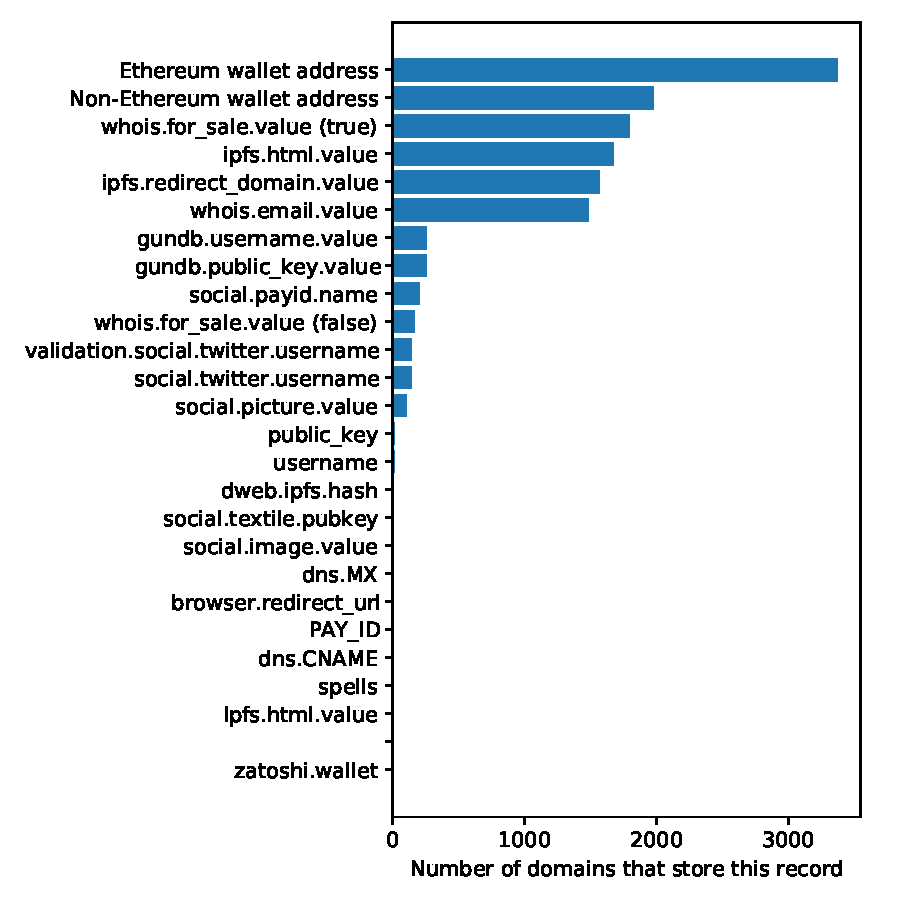
\includegraphics[width=3in]{figs/all_unstoppable_records.pdf}
	\caption{Records stored by Unstoppable Domains names.}
	\label{fig:unstoppable_records}
\end{figure}

%Describe the registry contract and the crawled domains (I did 
%crawl these didn't I?)

Like ENS, Unstoppable Domains uses Ethereum smart contracts as 
registrars. Unstoppable Domains names are divided into two systems. CNS 
(the Crypto Name System) contains all names with \texttt{.crypto} 
alt-TLDs, and has separate registry and resolver contracts. Later, Unstoppable 
added UNS 
(the Unstoppable Name System), which simplified name resolution by 
combining the resolver and registry contracts, and added several 
new alt-TLDs. Unstoppable Domains names never have to be renewed; they are 
purchased once and then owned indefinitely.

Like ENS names, Unstoppable Domains names are referenced by their hashes. We 
extracted all hashes from the UNS and CNS registry contracts 
by searching all of their transactions, and then found each 
hash's name and records by querying Unstoppable Domains' 
metadata endpoint.\footnote{	
\texttt{https://metadata.unstoppabledomains.com/metadata/}} 
This approach yielded a sample of 16,026 names. As with ENS, 
some names appear to exist in Unstoppable Domains that cannot 
be found by collecting transactions from these registry 
contracts. For example, it appears to be possible to store Unstoppable Domains 
names on the Polygon blockchain instead of Ethereum. We therefore note that our 
sample does not contain all of the names present in Unstoppable Domains.

Figure~\ref{fig:unstoppable_records} shows the distribution 
of record types found in the Unstoppable Domains names. As in 
ENS, the majority of names have wallet records rather than 
records that point to websites in any way. The second most common 
type of record is ``whois.for\_sale.value,'' showing that many 
names are seen as speculative assets. Unstoppable Domains also 
provides an easy way for users to link to IPFS records.

We performed a web crawl of all of the Unstoppable names that 
had records pointing to websites, whether IPFS records, 
traditional IP addresses, or traditional domains. We took 
screenshots of the 367 websites we arrived 
at, inspected them manually, and did not find any evidence of 
malware use. Most 
websites were personal sites, Web3-based business sites, or related to the sale 
or collection of NFTs. 



%Interestingly, we note that Unstoppable Domains has claimed that their naming 
%system cannot be easily abused, for two reasons. First, Unstoppable Domains 
%claims to police which domains may be sold. Unstoppable Domains claimed to 
%have 
%``prevented the registration of domains associated with known pirating 
%software 
%or other types of IP theft and fraud''~\cite{pegoraro_blockchain_2021}. 

